\chapter{Μεθοδολογία}
\label{ch:chapter3}

Στο κεφαλαίο αυτό παρουσιάζεται η μεθδολογία που ακολουθήθηκε κατά την διάρκεια της σύλλογης των δεδομένων των πειραμάτων με το \textlatin{GitHub Copilot} και με το \textlatin{GitHub Copilot Chat}. Αρχικά, η επιλογή της εφαρμογής πάνω στην οποία το \textlatin{GitHub Copilot} αξιολογήθηκε, περιγράφεται παρακάτω.

\section{Επιλογή Εφαρμογής}
\label{sec:app_selection}

Για την επιλογή της κατάλληλης εφαρμογής, λήφθηκαν οι παρακάτω παράμετροι υπ' όψιν:

\begin{itemize}
    \item \textbf{Πολυπλοκότητα της εφαρμογής:} Η εφαρμογή πρέπει να είναι αρκετά πολύπλοκη ώστε να απαιτεί την χρήση του \textlatin{GitHub Copilot} για την ανάπτυξη του κώδικα.
    \item \textbf{Τύπος της εφαρμογής:} Η εφαρμογή πρέπει να είναι μια ιδέα αντίστοιχη με τις υπόλoιπες υλοποιήσεις του κλάδου της Μηχανικής Λογισμικού και συγκεκριμένα της Ανάπτυξης Ιστότοπων \textlatin{\textbf{Web Development}}.
    \item \textbf{Γλώσσα της εφαρμογής και Τεχνολογική Στοίβα \textlatin{Technology Stack}:} Η επιλογή της Τεχνολογικής Στοίβας πρέπει να γίνει με βάση μοντέρνες τεχνολογίες και με ευρεία χρήση, προκειμένου το μοντέλο να έχει την περισσότερη εμπειρία και τις καλύτερες αποδόσεις, αλλά και να γίνεται μια αξιολόγηση με πραγματικά και εξελισσόμενα εργαλεία.
\end{itemize}

Με βάση τις παραπάνω παραμέτρους, επιλέχθηκε η ανάπτυξη μιας εφαρμογής η οποία θα αποτελείται από έναν ιστότοπο που θα παρέχει ένα μέσο δικτύωσης που αφορά τα βιντεοπαιχνίδια. Η εφαρμογή αυτή είχε ήδη αναπτυχθεί στα πλαίσια του μαθήματος ``Μηχανική Λογισμικού Ι'', επομένως οι βασικές ανάγκες και λειτουργίες της εφαρμογής είχαν καταγραφθεί. Η επιλογή αυτή έγινε προκειμένου η αξιολόγηση του κώδικα και των προτάσεων του \textlatin{GitHub Copilot} να μην έχει αλλαγές με βάση τις αλλαγές που προέκυψαν κατά τον σχεδιασμό της εφαρμογής. Η εφαρμογή αποτελείται από τρεις (3) βασικές λειτουργίες:

\begin{itemize}
    \item Κριτική παιχνιδιών και κοινοποίηση των κριτικών των χρηστών με τους υπόλοιπους χρήστες της εφαρμογής.
    \item Διαχείριση και κοινοποίηση λιστών \textlatin{(playlists)} από βιντεοπαιχνίδια με τους υπόλοιπους χρήστες της εφαρμογής.
    \item Δυνατότητα στον χρήστη να σχολιάσει τις κριτικές των άλλων χρηστών, καθώς και να ``ακολουθήσει'' άλλους χρήστες, λαμβάνοντας ειδοποιήσεις για τις ενέργειές τους.
\end{itemize}

Παρατίθεται το Σχεσιακό Διάγραμμα Οντοτήτων της εφαρμογής:

\begin{figure}[H]
  \begin{center}
    \resizebox*{!}{22cm}{%
        \rotatebox{270}{%
        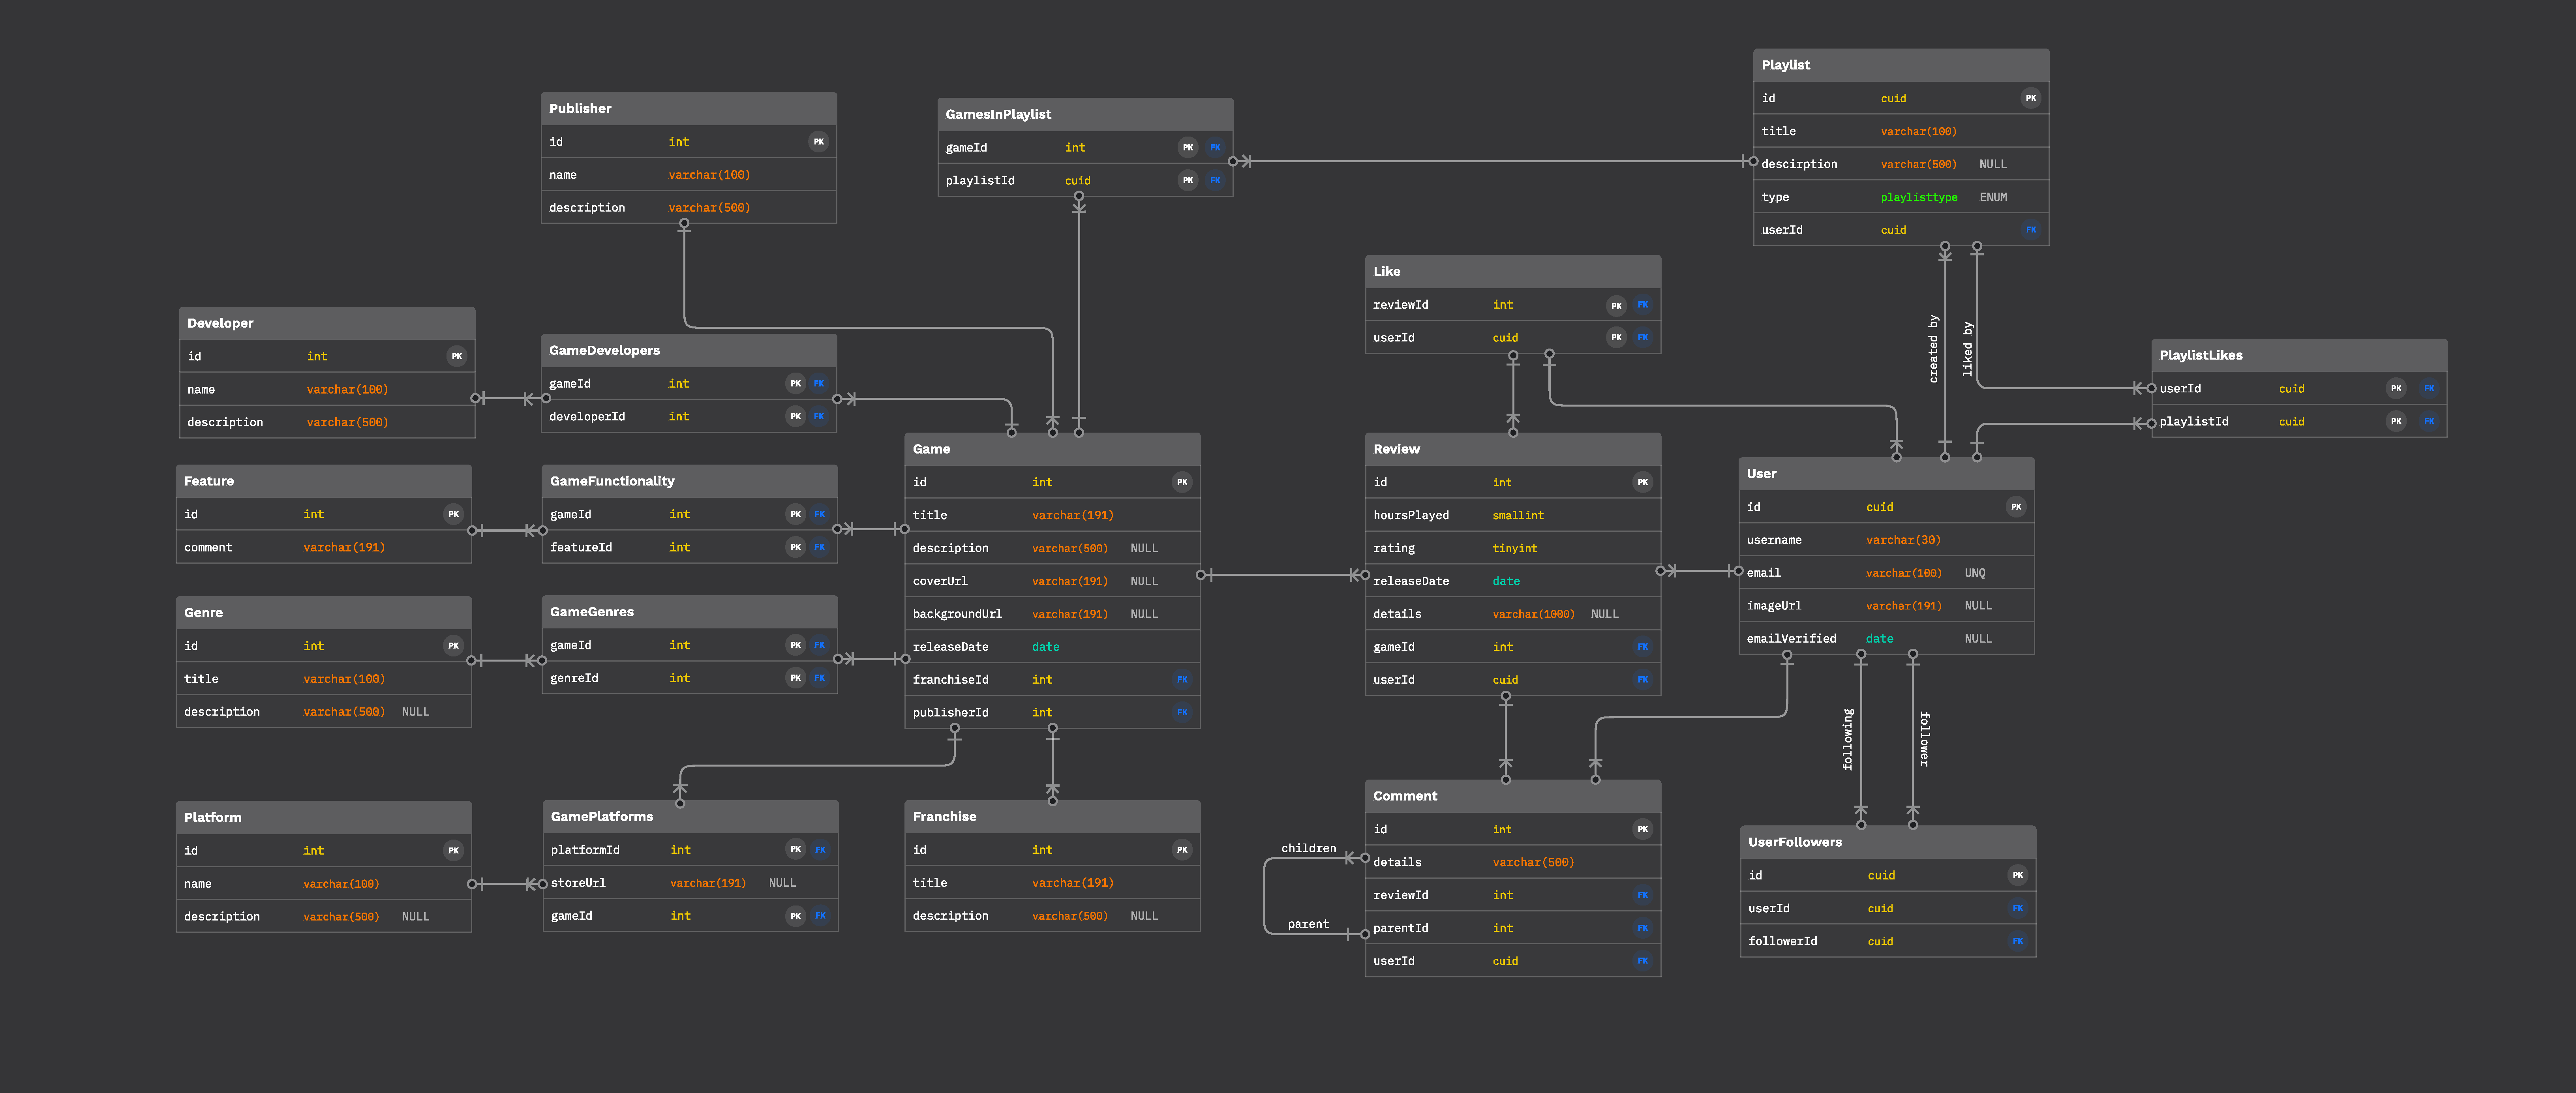
\includegraphics{Relational Database Diagram - Component Kit (Community).pdf}%
        }%
    }
    \caption{Σχεσιακό Διάγραμμα Οντοτήτων της εφαρμογής}
    \label{fig:RDD}
  \end{center}
\end{figure}
 
\subsection{Τεχνολογική Στοίβα \textlatin{Technology Stack}}
Η επιλογή της Τεχνολογικής Στοίβας έγινε με βάση την ευρεία χρήση των τεχνολογιών αυτών, την ευκολία στην ανάπτυξη και την ευκολία στην ενσωμάτωση του \textlatin{GitHub Copilot}. Η εφαρμογή αναπτύχθηκε με την χρήση των παρακάτω τεχνολογιών:
 
\begin{itemize}
    \item \textbf{Γλώσσα Προγραμματισμού}: Η εφαρμογή αναπτύχθηκε με την χρήση της γλώσσας προγραμματισμού \textlatin{Typescript} \cite{typescript}, ενός συντακτικού υπερσυνόλου της γλώσσας \textlatin{JavaScript} \cite{javascript}, μια από τις πιο διαδομένες γλώσσες προγραμματισμού στον κόσμο. \cite{tiobe, languagechart}
    \item \textbf{Εμπρόσθια Ανάπτυξη (\textlatin{Frontend Development}):} Η εμπρόσθια ανάπτυξη της εφαρμογής έγινε με την χρήση της \textlatin{React} \cite{react}, μιας βιβλιοθήκης της \textlatin{JavaScript} για την ανάπτυξη διεπαφών χρήστη. Συγκεκριμένα, χρησιμοποιήθηκε το πλαίσιο εργασίας \textlatin{Next.js} \cite{nextjs}, το οποίο παρέχει δυνατότητες όπως την προ-φόρτωση των σελίδων, την δυνατότητα δημιουργίας στατικών ιστοσελίδων, και την δυνατότητα δημιουργίας δυναμικών ιστοσελίδων, αποτελώντας ένα από τα πιο ευρέως χρησιμοποιημένα πλαίσια εργασίας.
    \item \textbf{Πίσω Ανάπτυξη (\textlatin{Backend Development}):} Η πίσω ανάπτυξη της εφαρμογής έγινε με την χρήση της βιβλιοθήκης \textlatin{tRPC} \cite{trpc}, μιας βιβλιοθήκης που παρέχει την δυνατότητα δημιουργίας \textlatin{API} με την χρήση της γλώσσας \textlatin{Typescript}. Η βάση δεδομένων της εφαρμογής αποθηκεύτηκε σε μια βάση δεδομένων \textlatin{MySQL} \cite{mysql}, μιας από τις πιο διαδεδομένες σχεσιακές βάσεις δεδομένων. Tο εργαλείο της Αντικειμενο-σχεσιακής Απεικόνισης \textlatin{(ORM)} που χρησιμοποιήθηκε ήταν το \textlatin{Prisma} \cite{prisma}, το οποίο παρέχει την δυνατότητα δημιουργίας απλών και ασφαλών ερωτημάτων \textlatin{(queries)} στην βάση δεδομένων. To σύστημα διαχείρισης της ταυτότητας των χρηστών \textlatin{(authentication)} και των δικαιωμάτων τους \textlatin{(authorization)} υλοποιήθηκε με την χρήση της βιβλιοθήκης \textlatin{NextAuth.js} \cite{nextauth}.
    \item \textbf{Έλεγχος Λογισμικού (\textlatin{Software Testing}):} Για τον έλεγχο της λειτουργίας του παραγόμενου κώδικα, χρησιμοποιήθηκε το πλαίσιο εργασίας \textlatin{Jest} \cite{jest}, το οποίο παρέχει την δυνατότητα δημιουργίας και εκτέλεσης δοκιμαστικών συνόλων κώδικα, με σκοπό την εξασφάλιση της άρτιας λειτουργίας του κώδικα. \cite{Jacobson1999,irena2008,swebok2004,miller1981,shaw1990}
\end{itemize}

Η παραπάνω στοίβα ονομάστηκε \textlatin{T3 stack}, έχοντας πλέον δημιουργήσει μια μεγάλη κοινώτητα στον κλάδο της ανάπυτξης ιστότοπων και της ανάπτυξης λογισμικού. \cite{t3repo}

\section{Συλλογή Δεδομένων}

Για την συλλογή των δεδομένων, αρχικά δημιουργήθηκε ο σκελετός της βάσης κώδικα \textlatin{(codebase)}, καθώς και μια λειτουργικότητα της εφαρμογής, μαζί με τα αντίστοιχα αρχεία ελέγχου της λειρουγίας του κώδικα. Η λειτουργικότητα που επιλέχθηκε να αναπτυχθεί χωρίς την χρήση του μοντέλου ήταν αυτής της σειράς του βιντεοπαιχνιδιού \textlatin{(Franchise)}. Η επιλογή έγινε γιατί η λειτουργικότητα αυτή ήταν αρκετά απλή, καθώς η σειρά έχει μόνο σχέσεις 1:Μ με οντότητα του βιντεοπαιχνιδιού \textlatin{(Game)} \ref{fig:RDD}. 

Με αυτό τον τρόπο, δημιουργήθηκαν μέθοδοι για την δημιουργία, την ανάγνωση, την ενημέρωση και την διαγραφή των σειρών του βιντεοπαιχνιδιού \textlatin{(CRUD)}, καθώς και έλεγχοι για την σωστή εκτέλεση αυτών, με βάση την ταυτοποίηση και των δικαιωμάτων των χρηστών. Σκοπός της προεργασίας αυτής ήταν η αξιολόγηση του κατά πόσο το μοντέλο θα ακολουθούσε τις κατευθυντήριες γραμμές που ορίστηκαν από τον προγραμματιστή.

\subsection{Διαδικασία Συλλογής Δεδομένων}
Για την καλύτερη μορφή και κατηγοριοποίηση των δεδομένων, η κάθε προτροπή χωρίστηκε σε τέσσερις (4) κατηγορίες, με βάση τo είδος της:

\begin{itemize}
  \item \textbf{Γλώσσας (\textlatin{Language})} Προτροπές που αφορούν ερωτήσεις για την γλώσσα προγραμματισμού (συντακτικό, δομή).
  \item \textbf{Πίσω  Ανάπτυξης (\textlatin{Backend})} Προτροπές που αφορούν ερωτήσεις για την ανάπτυξη του \textlatin{API} της εφαρμογής.
  \item \textbf{Ελέγχου (\textlatin{Testing})} Προτροπές που αφορούν ερωτήσεις για την ανάπτυξη ελέγχου για τις μεθόδους που έχουν γραφτεί.
  \item \textbf{Άλλες} Προτροπές που αφορούν ερωτήσεις που δεν σχετίζονται με την συγγραφή κώδικα (για την λειτουργικότητα του \textlatin{GitHub Copilot}, για την δομή των απαντήσεών του, τυχόν λάθη από πλευρά του προγραμματιστή κατά την σύνταξη της προτροπής).
\end{itemize}

Πέρα από την αρχική κατηγοριοποίηση των προτροπών, η κάθε προτροπή επίσης κατηγοριοποίηθηκε περαιτέρω, με το κάθε θέμα της ερώτησης,  

Για την συλλογή των δεδομένων, δημιουργήθηκε μια περσόνα ενός προγραμματιστή για το μοντέλο \cite{zhou2024sotopia,AitBaha2023, xu2023expertprompting}, με τους κανόνες να ακολουθεί κάθε του απάντηση μια συγκεκριμένη δομή. Ζητήθηκε από το μοντέλο να αρχίζει κάθε μήνυμα με το θέμα της ερώτησης 

